\documentclass[04_projectProcess.tex]{subfiles}
\begin{document}
    \subsection{Soldering and Implementation Process}
    \begin{flushleft}
        After getting to know the material, soldering and programming were the next steps(see Figure \ref{fig:solderingProcess} and \ref{fig:UMLDiagram}).
        An Arduino Pro Mini \cite{arduinoProMini}, some resistors (like 
        1M\si{\ohm} resistors), copper foil and a Neopixel WS2812 have been used. \\      
        
        \begin{figure}[H]
            \centering
            \begin{subfigure}{.45\textwidth}
                \centering
                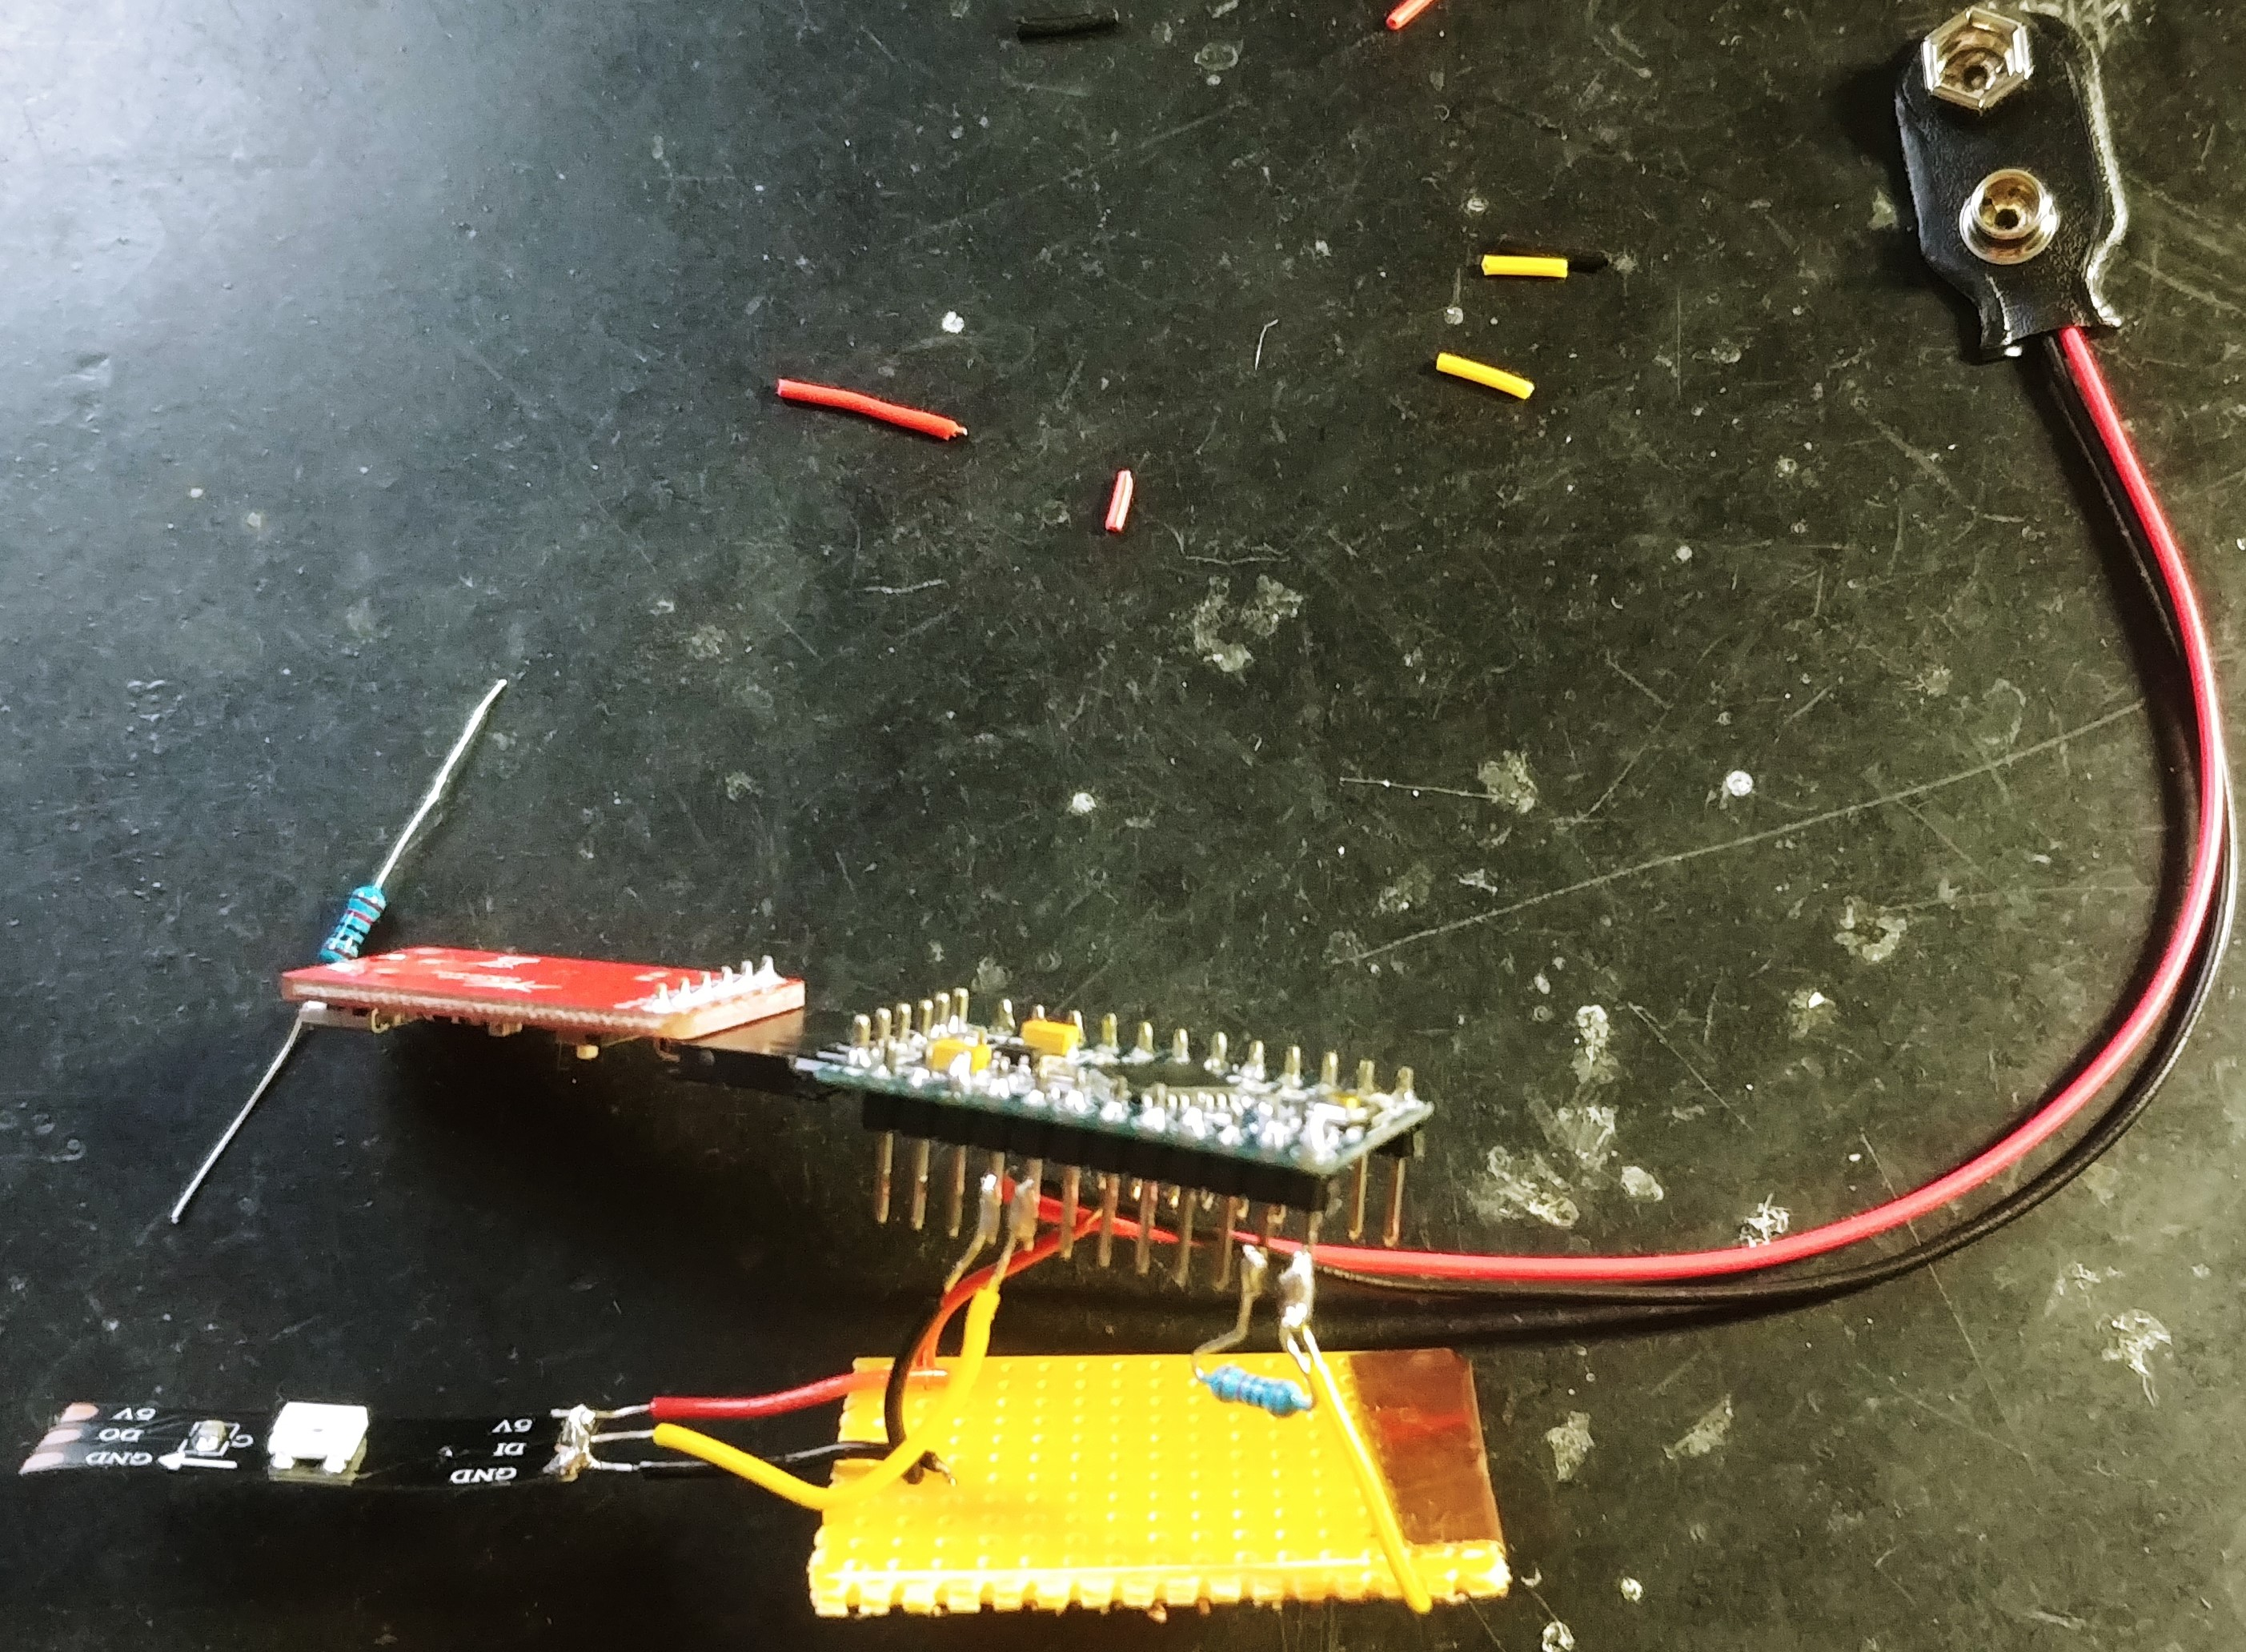
\includegraphics[width=0.8\linewidth]{images/programmingProcess/solderingProcess.jpg}
                \caption{Shows a testing soldering.}
                \label{fig:solderingProcess_0}
                \vspace{6mm}
            \end{subfigure}
            \begin{subfigure}{.45\textwidth}
                \centering
                \includegraphics[scale=0.065]{images/programmingProcess/Soldering_Process_1.jpg}
                \caption{Shows the soldering process of the RGB-LEDs from the top.}
                \label{fig:solderingProcess_1}
                \vspace{6mm}
            \end{subfigure}
            \hspace{1mm}
            \begin{subfigure}{.45\textwidth}
                \centering
                \includegraphics[scale=0.051]{images/programmingProcess/Soldering_Process_2.jpg}
                \caption{Shows the soldering process of the RGB-LEDs from the bottom.}
                \label{fig:solderingProcess_2}
                \vspace{6mm}
            \end{subfigure}
            \begin{subfigure}{.45\textwidth}
                \centering
                \includegraphics[width=0.65\linewidth]{images/programmingProcess/finalSoldering.jpg}
                \caption{Shows the outcome of the soldering process.} 
                \label{fig:finalSoldering}
                \vspace{6mm}
            \end{subfigure}
            \begin{subfigure}{.45\textwidth}
                \centering
                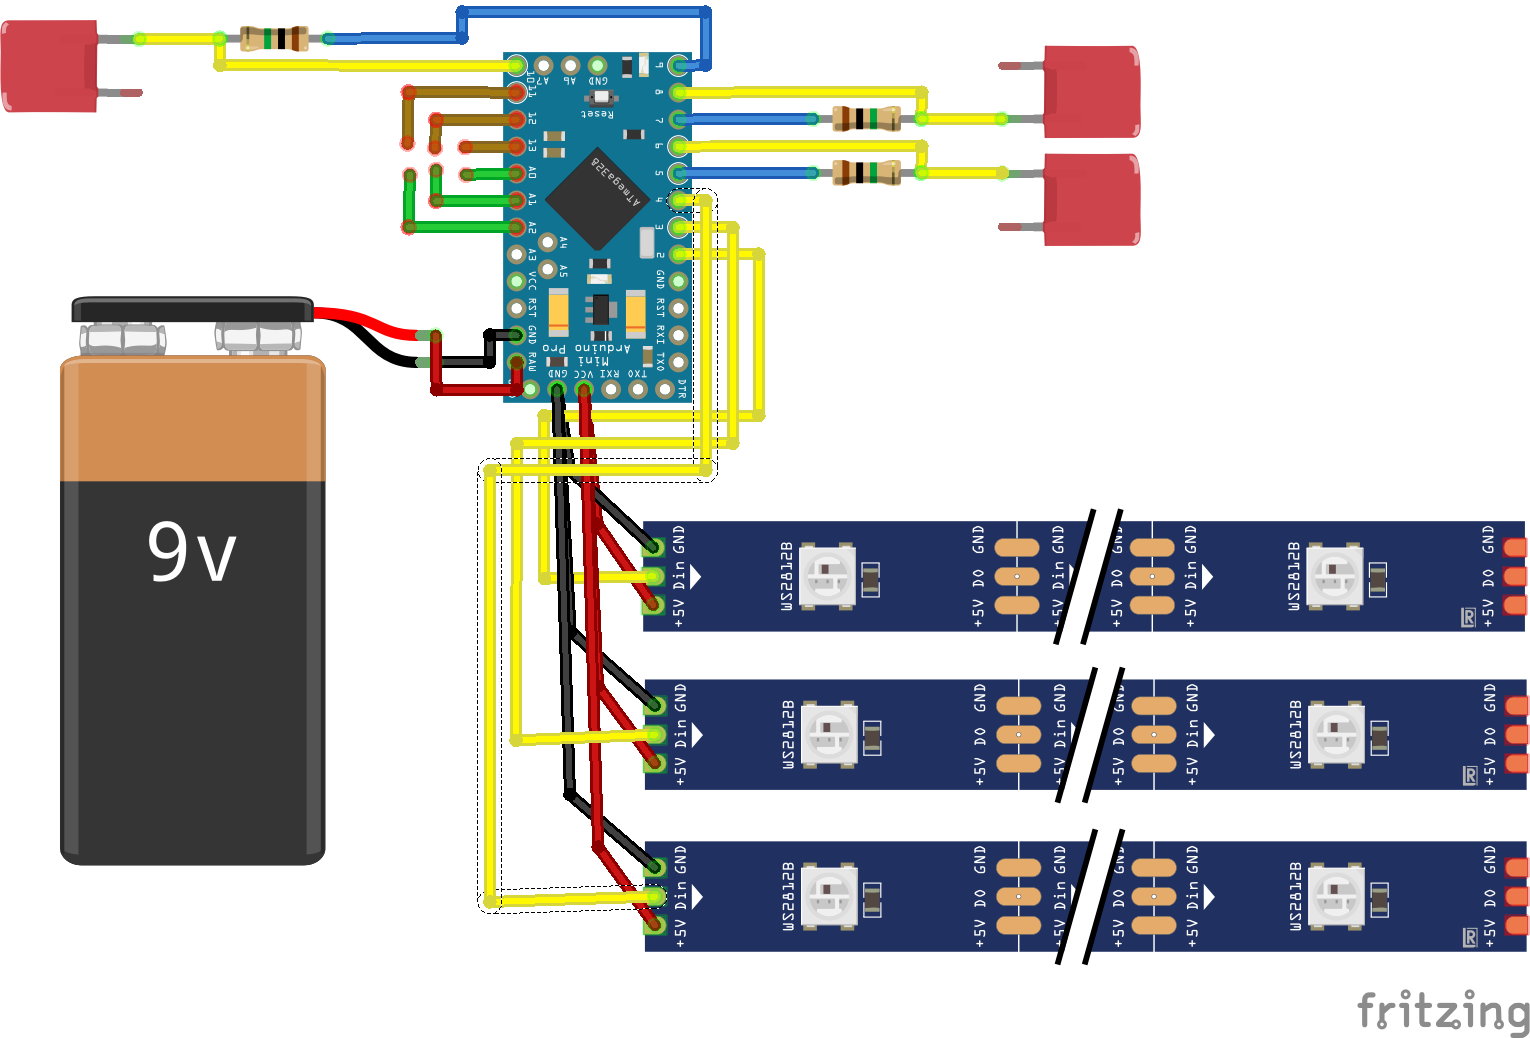
\includegraphics[width=0.8\linewidth]{images/programmingProcess/sensorLinks.png}
                \caption{Shows the links between the microcontroller and the LEDs and copper foil that is 
                used as a capacitive sensor. This image has been done by Frizing. \cite{fritzing}}
                \label{fig:solderingProcess_3}
                \vspace{6mm}
            \end{subfigure}
            \caption{Shows the soldering process and linking.}
            \label{fig:solderingProcess}
        \end{figure}

        \noindent
        To program every functionality, the Arduino IDE  has been used. The programming language 
        is C++ with some additional Arduino specific function and global variables \cite{introductionArduino}. 
        Different classes have been programmed that specify different functionalities or sensor 
        of this project \cite{arduinoClasses}. The following UML diagram shows the final code 
        structure of the project (see Figure \ref{fig:UMLDiagram}).

        \begin{figure}[H]
            \centering
            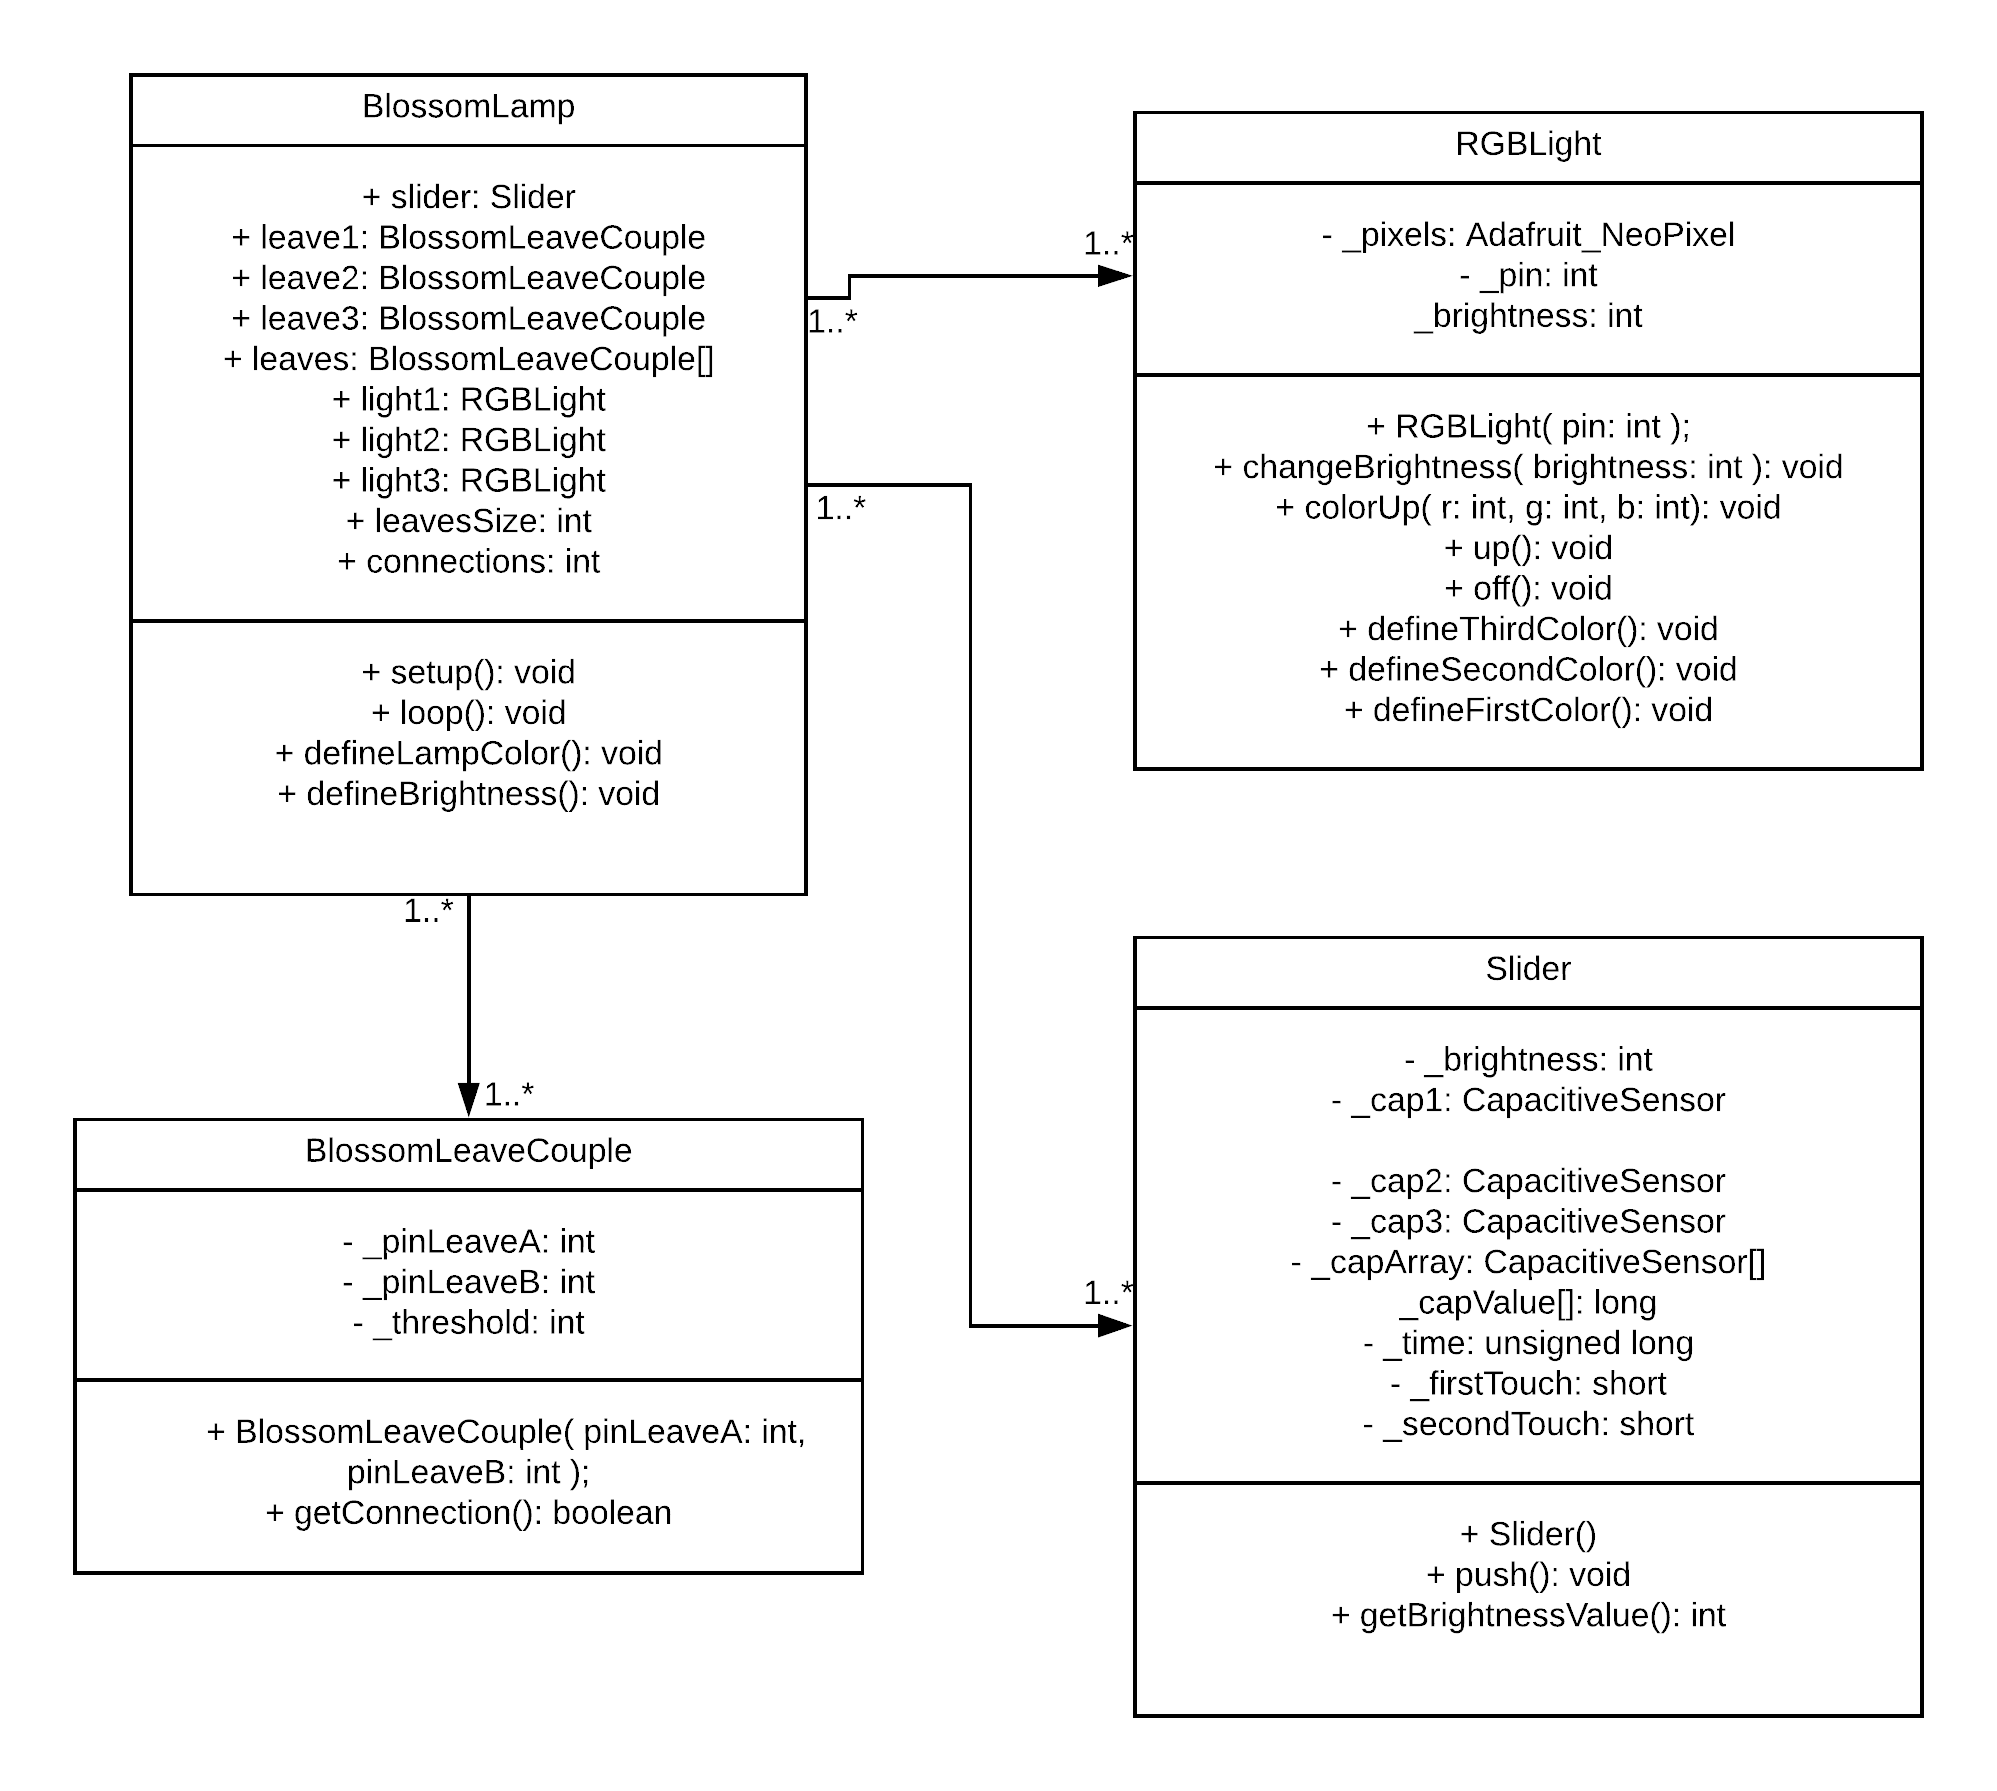
\includegraphics[width=0.8\linewidth]{images/programmingProcess/BlossomLamp_UML.png}
            \caption{Shows the code stucture and UML diagram of the project.}
            \label{fig:UMLDiagram}
        \end{figure}

        \noindent
        The resistors and the copper foil are used to build a capacitive sensor. \cite{Badger2019} 
        If the user pushes the capacitive sensor, the microcontroller can sense it. This functionality
        will be used to create an analog slider. The slider has been programmed, so users can change the 
        brightness. However, just three capacitive sensors have been programmed because of the Arduino 
        Pro Mini doesn't have enough digital pins for every sensor. However, three capacitive sensors can show 
        the concept and the initial idea. The soldering process of capacitive sensors can be found in 
        Figure \ref{fig:finalSoldering}. \\~\\

        \noindent
        The Neopixel WS2812 will be used to make the lamp shine in different colors. \cite{Burgess2019} 
        To get close to the initial idea, three more holes have been drilled inside the base. 
        This is the place for every LED (Neopixel WS2812). Before putting them inside, cables had to be 
        soldered, so the LEDs could be tested(see \ref{fig:solderingProcess_1}).\\~\\

        \noindent
        Furthermore, the leaf connections have been implemented, so the system can detect if 
        the users pull a blossom. This process changes the color of the lamp.

        \noindent
        The final code can be found on GitHub:  
        https://github.com/ChrisHeiden/Tangible\_Interfaces\_Project
    \end{flushleft}
\end{document}
